\documentclass[11pt, a4paper]{article}
\usepackage{pdfpages}
\usepackage{parallel}
\usepackage[T2A]{fontenc}
%\usepackage{ucs}
\usepackage[utf8]{inputenc}
\usepackage[english,russian]{babel}
\usepackage{hyperref}
\usepackage{rotating}
\usepackage[inner=2cm,top=1.8cm,outer=2cm,bottom=2.3cm,nohead]{geometry}
%\usepackage{listings}
\usepackage{graphicx}
\usepackage{wrapfig}
\usepackage{longtable}
\usepackage{indentfirst}
\usepackage{array}
\usepackage{tikzsymbols}
\usepackage{soul}
\usepackage[ruled,vlined]{algorithm2e}
\usepackage{qrcode}
\counterwithout{figure}{section} 

\usepackage{url}
\makeatletter
\g@addto@macro{\UrlBreaks}{\UrlOrds}
\makeatother

\newcolumntype{P}[1]{>{\raggedright\arraybackslash}p{#1}}
\frenchspacing
%\usepackage{fixltx2e} %text sub- and superscripts
\usepackage{icomma} % коскі ў матэматычным рэжыме
%\PreloadUnicodePage{4}

\newcommand{\longpage}{\enlargethispage{\baselineskip}}
\newcommand{\shortpage}{\enlargethispage{-\baselineskip}}

\def\switchlang#1{\expandafter\csname switchlang#1\endcsname}
\def\switchlangbe{
\let\saverefname=\refname%
\def\refname{Літаратура}%
\def\figurename{Іл.}%
}
\def\switchlangru{
\let\saverefname=\refname%
\let\savefigurename=\figurename%
\def\refname{Литература}%
\def\figurename{Рис.}%
}
\def\switchlangen{
\let\saverefname=\refname%
\def\refname{References}%
\def\figurename{Fig.}%
}

\hyphenation{admi-ni-stra-tive}
\hyphenation{ex-pe-ri-ence}
\hyphenation{fle-xi-bi-li-ty}
\hyphenation{Py-thon}
\hyphenation{ma-the-ma-ti-cal}
\hyphenation{re-ported}
\hyphenation{imp-le-menta-tions}
\hyphenation{pro-vides}
\hyphenation{en-gi-neering}
\hyphenation{com-pa-ti-bi-li-ty}
\hyphenation{im-pos-sible}
\hyphenation{desk-top}
\hyphenation{elec-tro-nic}
\hyphenation{com-pa-ny}
\hyphenation{de-ve-lop-ment}
\hyphenation{de-ve-loping}
\hyphenation{de-ve-lop}
\hyphenation{da-ta-ba-se}
\hyphenation{plat-forms}
\hyphenation{or-ga-ni-za-tion}
\hyphenation{pro-gramming}
\hyphenation{in-stru-ments}
\hyphenation{Li-nux}
\hyphenation{sour-ce}
\hyphenation{en-vi-ron-ment}
\hyphenation{Te-le-pathy}
\hyphenation{Li-nux-ov-ka}
\hyphenation{Open-BSD}
\hyphenation{Free-BSD}
\hyphenation{men-ti-on-ed}
\hyphenation{app-li-ca-tion}

\def\progref!#1!{\texttt{#1}}
\renewcommand{\arraystretch}{2} %Іначай формулы ў матрыцы зліпаюцца з лініямі
\usepackage{array}

\def\interview #1 (#2), #3, #4, #5\par{

\section[#1, #3, #4]{#1 -- #3, #4}
\def\qname{LVEE}
\def\aname{#1}
\def\q ##1\par{{\noindent \bf \qname: ##1 }\par}
\def\a{{\noindent \bf \aname: } \def\qname{L}\def\aname{#2}}
}

\def\interview* #1 (#2), #3, #4, #5\par{

\section*{#1\\{\small\rm #3, #4. #5}}
\ifx\ParallelWhichBox\undefined%
    \addcontentsline{toc}{section}{#1, #3, #4}%
\else%
\ifnum\ParallelWhichBox=0%
    \addcontentsline{toc}{section}{#1, #3, #4}%
\fi\fi%

\def\qname{LVEE}
\def\aname{#1}
\def\q ##1\par{{\noindent \bf \qname: ##1 }\par}
\def\a{{\noindent \bf \aname: } \def\qname{L}\def\aname{#2}}
}

\newcommand{\interviewfooter}[1]{
\vskip 1em
\noindent \textit{#1}
}

\AtEndDocument{\vfill\centering \qrcode{https://github.com/fiowro/mouses/blob/main/\jobname.pdf}}

\switchlang{en}
\begin{document}

\title{1989 "--- Kraft trackball}
\date{}
\maketitle
\selectlanguage{english}
The Kraft trackball, also known as the Kraft TripleTrack \cite{triple}, is a device developed in the late 80s by Kraft Systems and released simultaneously for several computer families: IBM PC, Atari ST, Commodore 64 and Amiga. Trackball features include a key lock switch for selection and a detachable pedal.

\begin{figure}[h]
    \centering
    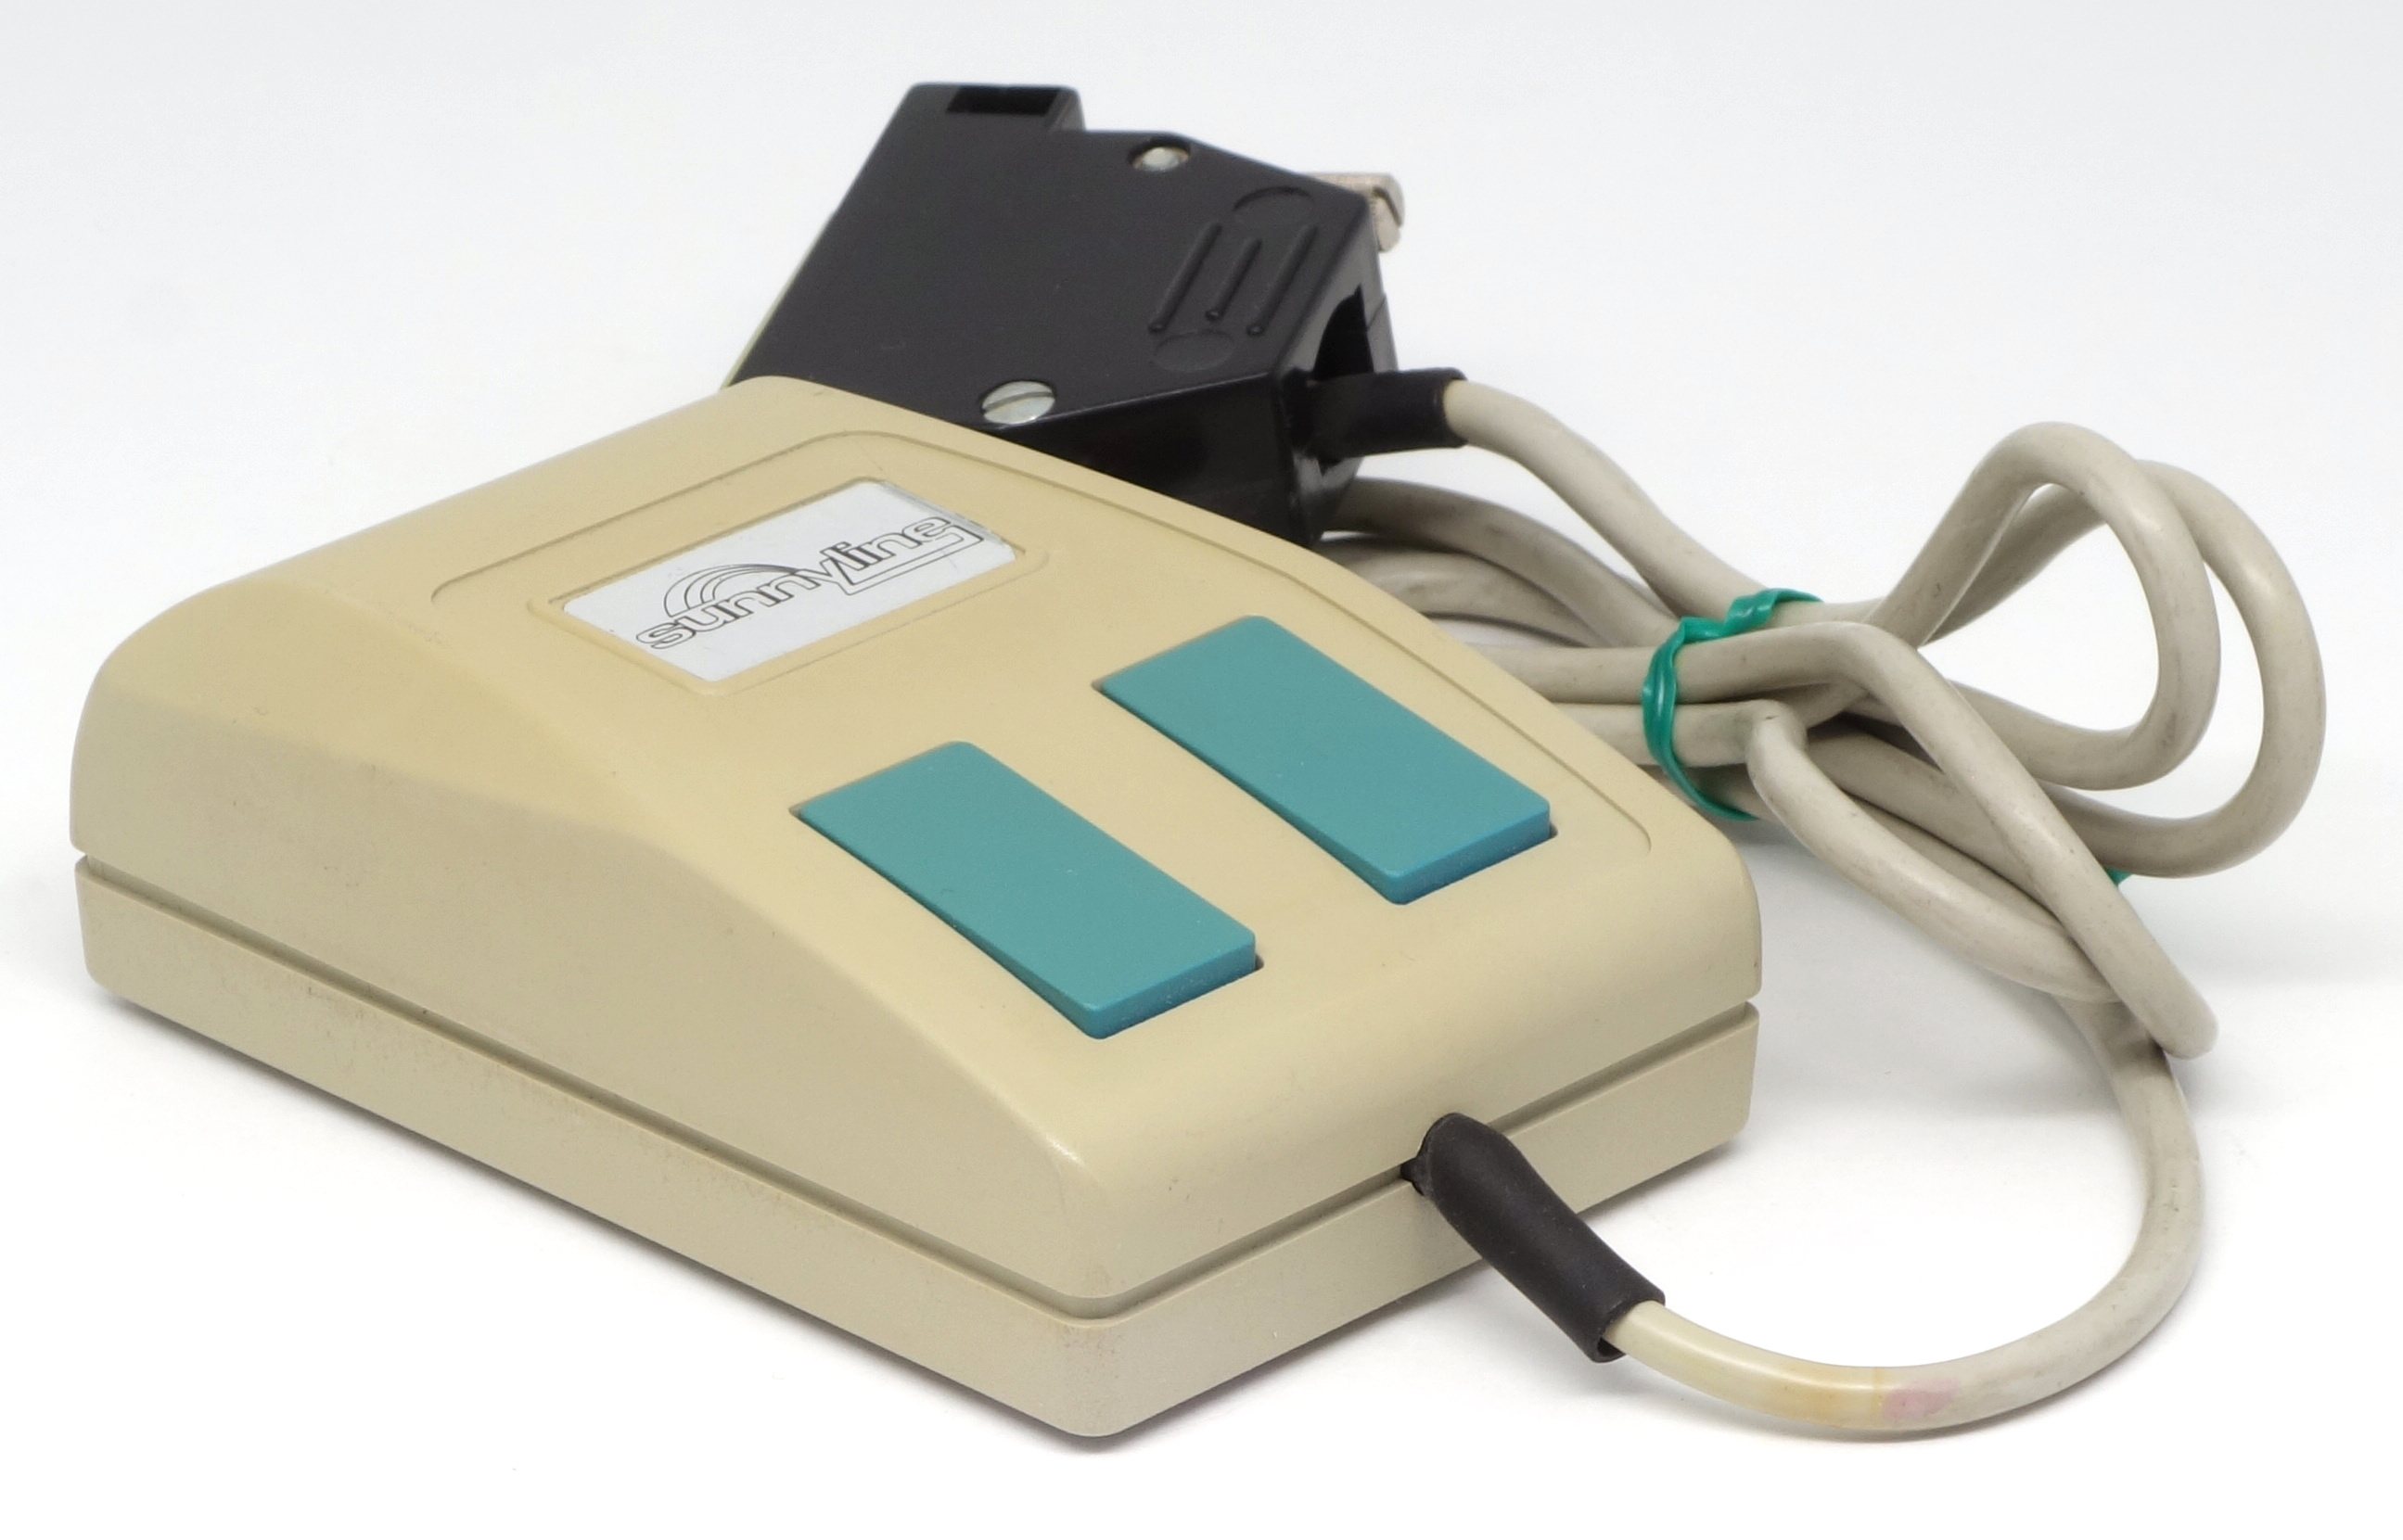
\includegraphics[scale=0.4]{1989_kraft_trackball/pic_30.jpg}
    \caption{Kraft trackball}
    \label{fig:KraftPhoto}
\end{figure}

The Kraft trackball has a symmetrical body and is therefore suitable for both left and right handers. Three buttons are located on the part of the device closest to the user, so the trackball does not offer any support under the wrist. The center button acts like a standard right mouse button. Buttons actuate high-quality switches with a distinct click; however, due to the large travel, the button caps go deeper into the case when pressed, making them harder to press with the thumb.

\begin{figure}[h]
    \centering
    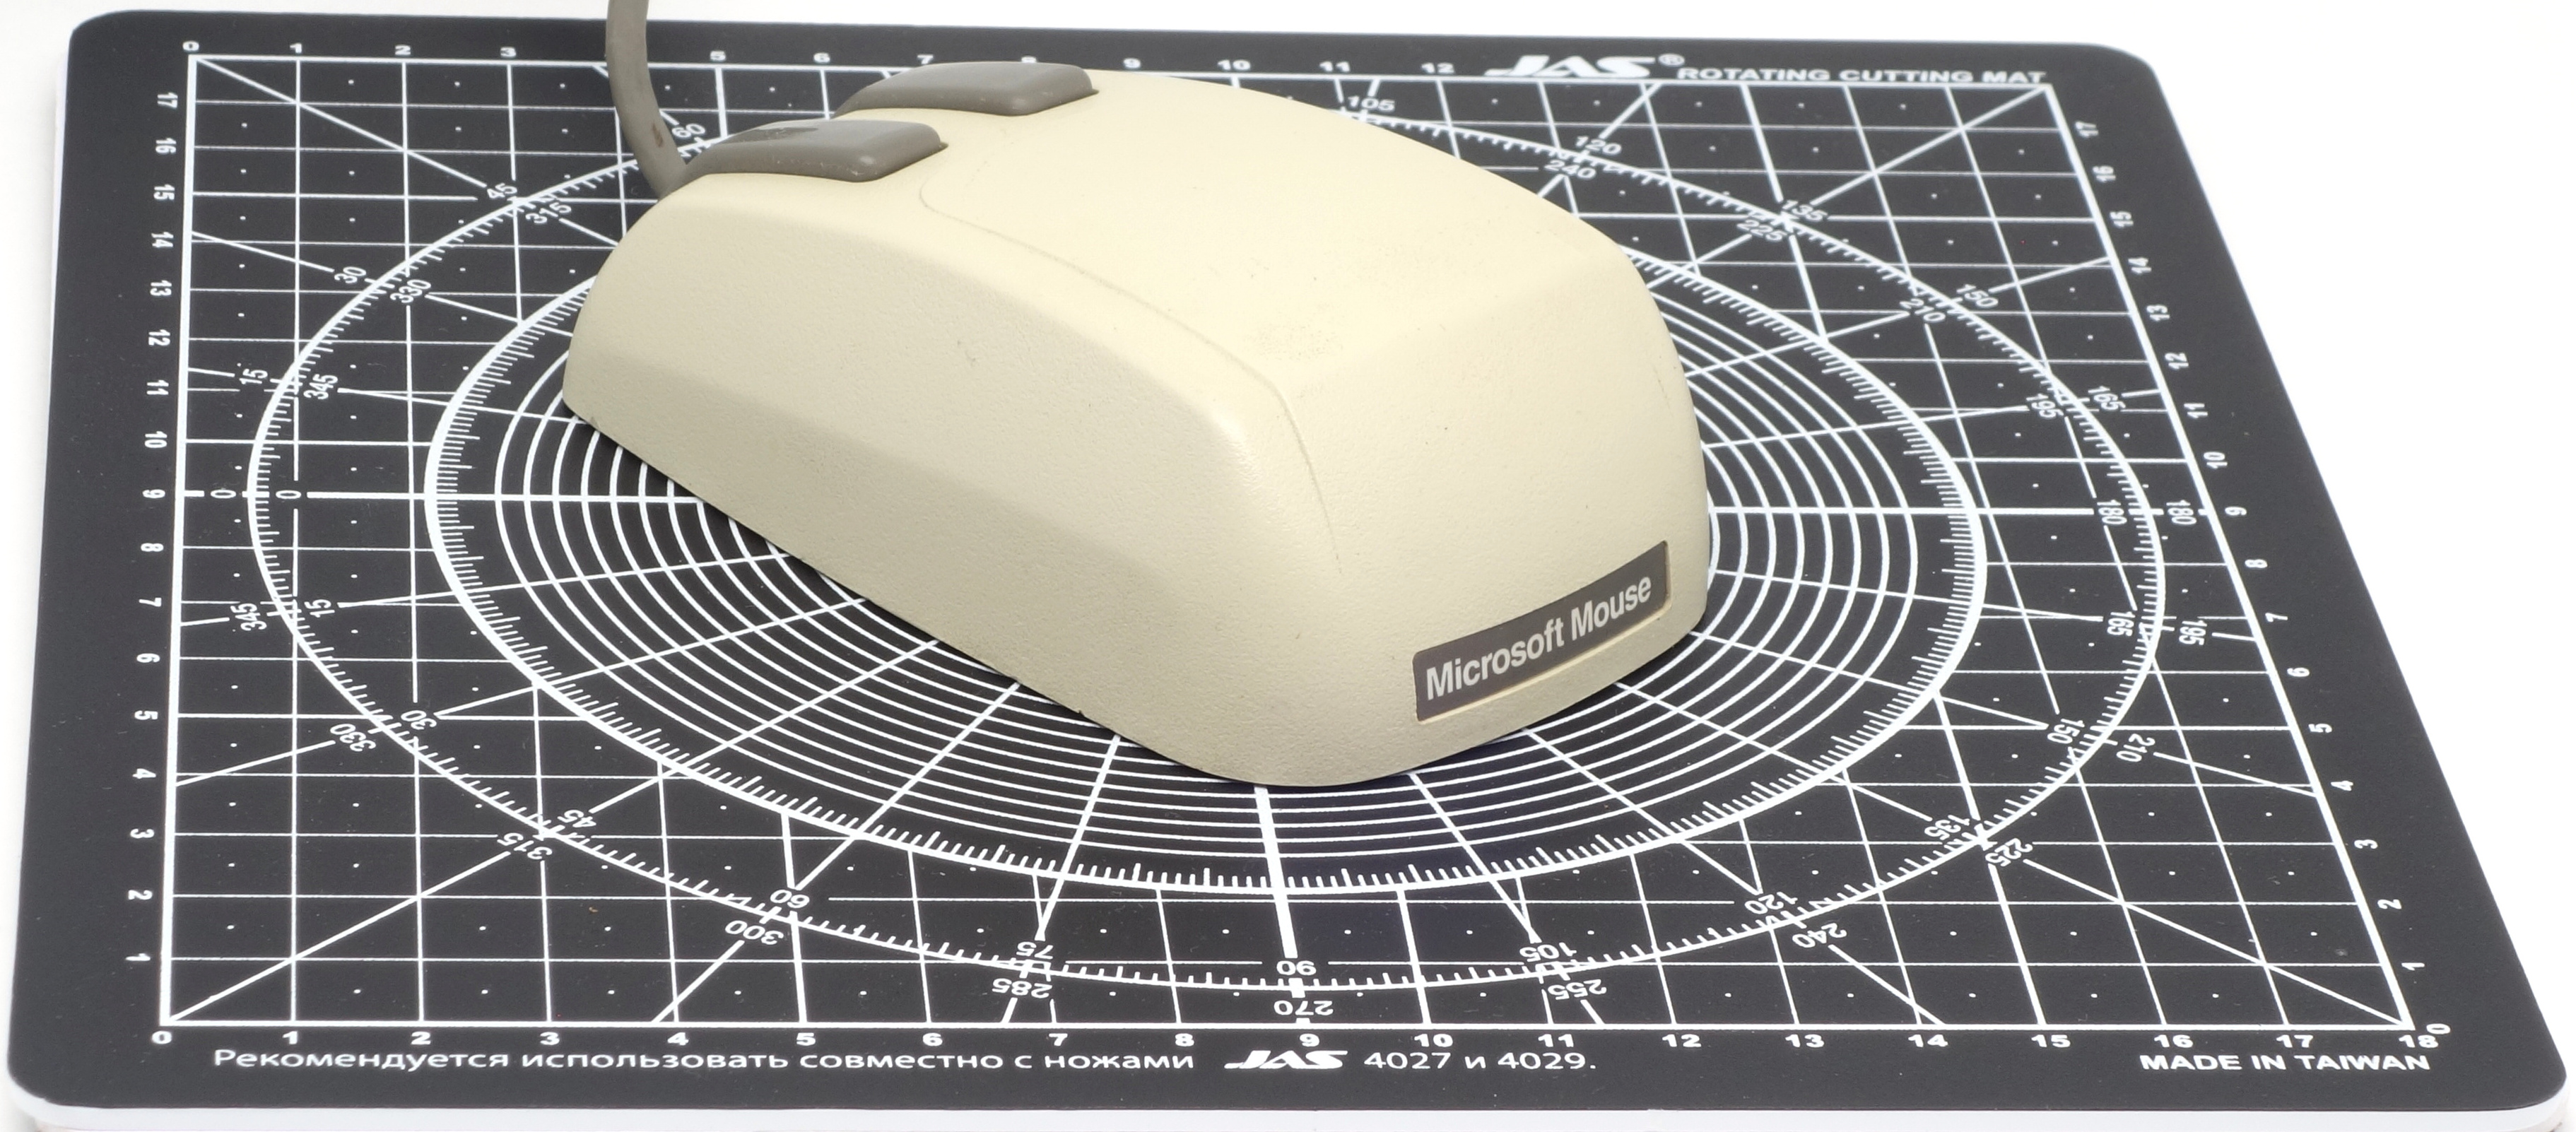
\includegraphics[scale=0.25]{1989_kraft_trackball/size_30.jpg}
    \caption{Kraft trackball on a graduated pad with a grid step of 1~cm}
    \label{fig:KraftSize}
\end{figure}

The ball has good moveability, so the device has no problems in controlling the cursor. At the same time, the part with the ball is somewhat raised above the buttons, which is an advantage in terms of ergonomics.

As noted in \cite{Hudnall}, the device was distinguished by the ease of installation of the bundled software, as well as two problems in cursor control: the buttons are harder to press than, for example, the buttons on popular mouse models, and sometimes the ball slips (the cursor remains in place). The latter problem can be solved by the user with a quick back and forth movement of the ball. In general, it's pretty easy to move the cursor around the screen by placing your middle finger on the ball and your thumb on the leftmost button (figure \ref{fig:KraftHand}). Using the right or middle button is less anatomically natural, more difficult to get used to, and fortunately for the user, it was not required as often in the late 80s.

\begin{figure}[h]
    \centering
    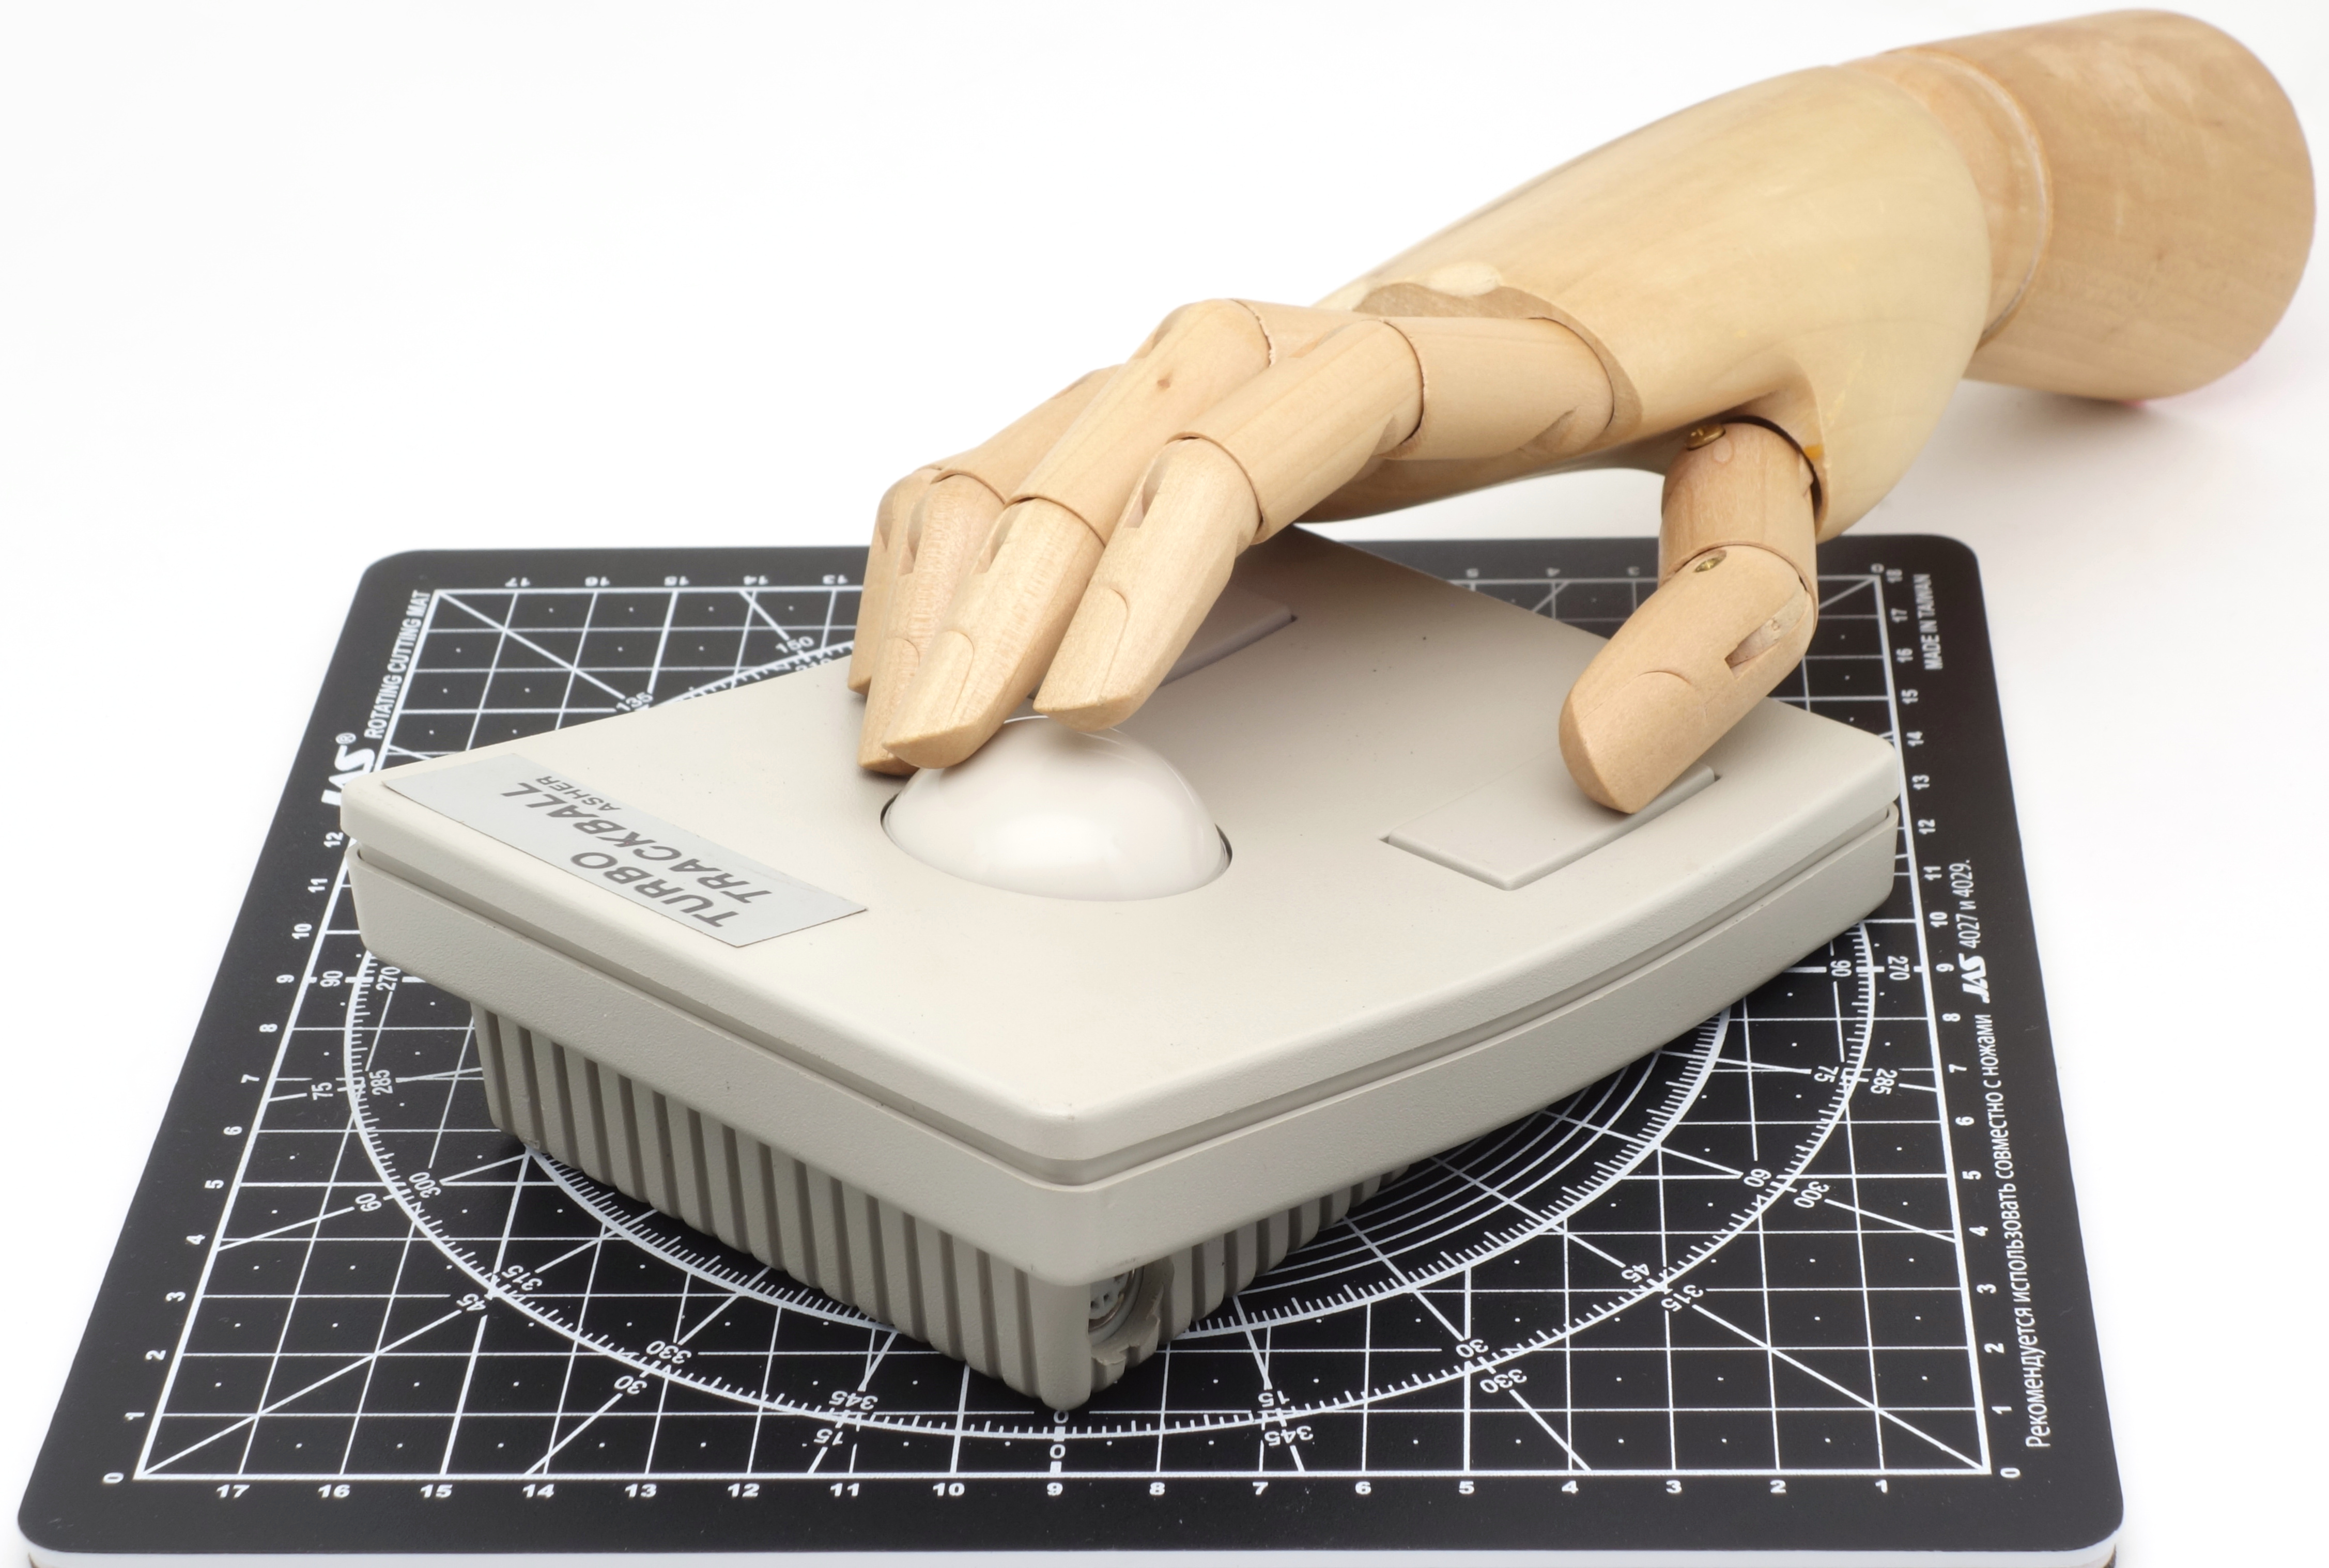
\includegraphics[scale=0.25]{1989_kraft_trackball/hand_30.jpg}
    \caption{Kraft trackball with a human hand model}
    \label{fig:KraftHand}
\end{figure}

To facilitate the operations of dragging objects, as well as selecting text by clicking and dragging, the device has a fourth button located behind the ball on the left. It works like a left button, but is implemented on the basis of a latching switch, so it is blocked in the pressed state until the next press. The location of this button suggests that it is designed to be pressed with the index finger. Given its location, small size, and shape, users probably didn't press it too often.

A unique accessory that came with the Kraft trackball is the foot pedal (figures \ref{fig:KraftPedal}). It connects to the back of the trackball using a standard RJ-11 telephone cable and is a solid rectangular box 1.5 inches high, 2 inches wide, and 4 inches long. Pressing the pedal is the same as pressing the left trackball button. According to the review presented in \cite{kraftwithpedal}, in actual use the pedal can almost completely replace the left button.

\begin{figure}[h]
    \centering
    \includegraphics[scale=0.4]{1990_kraft_toptrack/pedal_30.jpg} \hfill 
    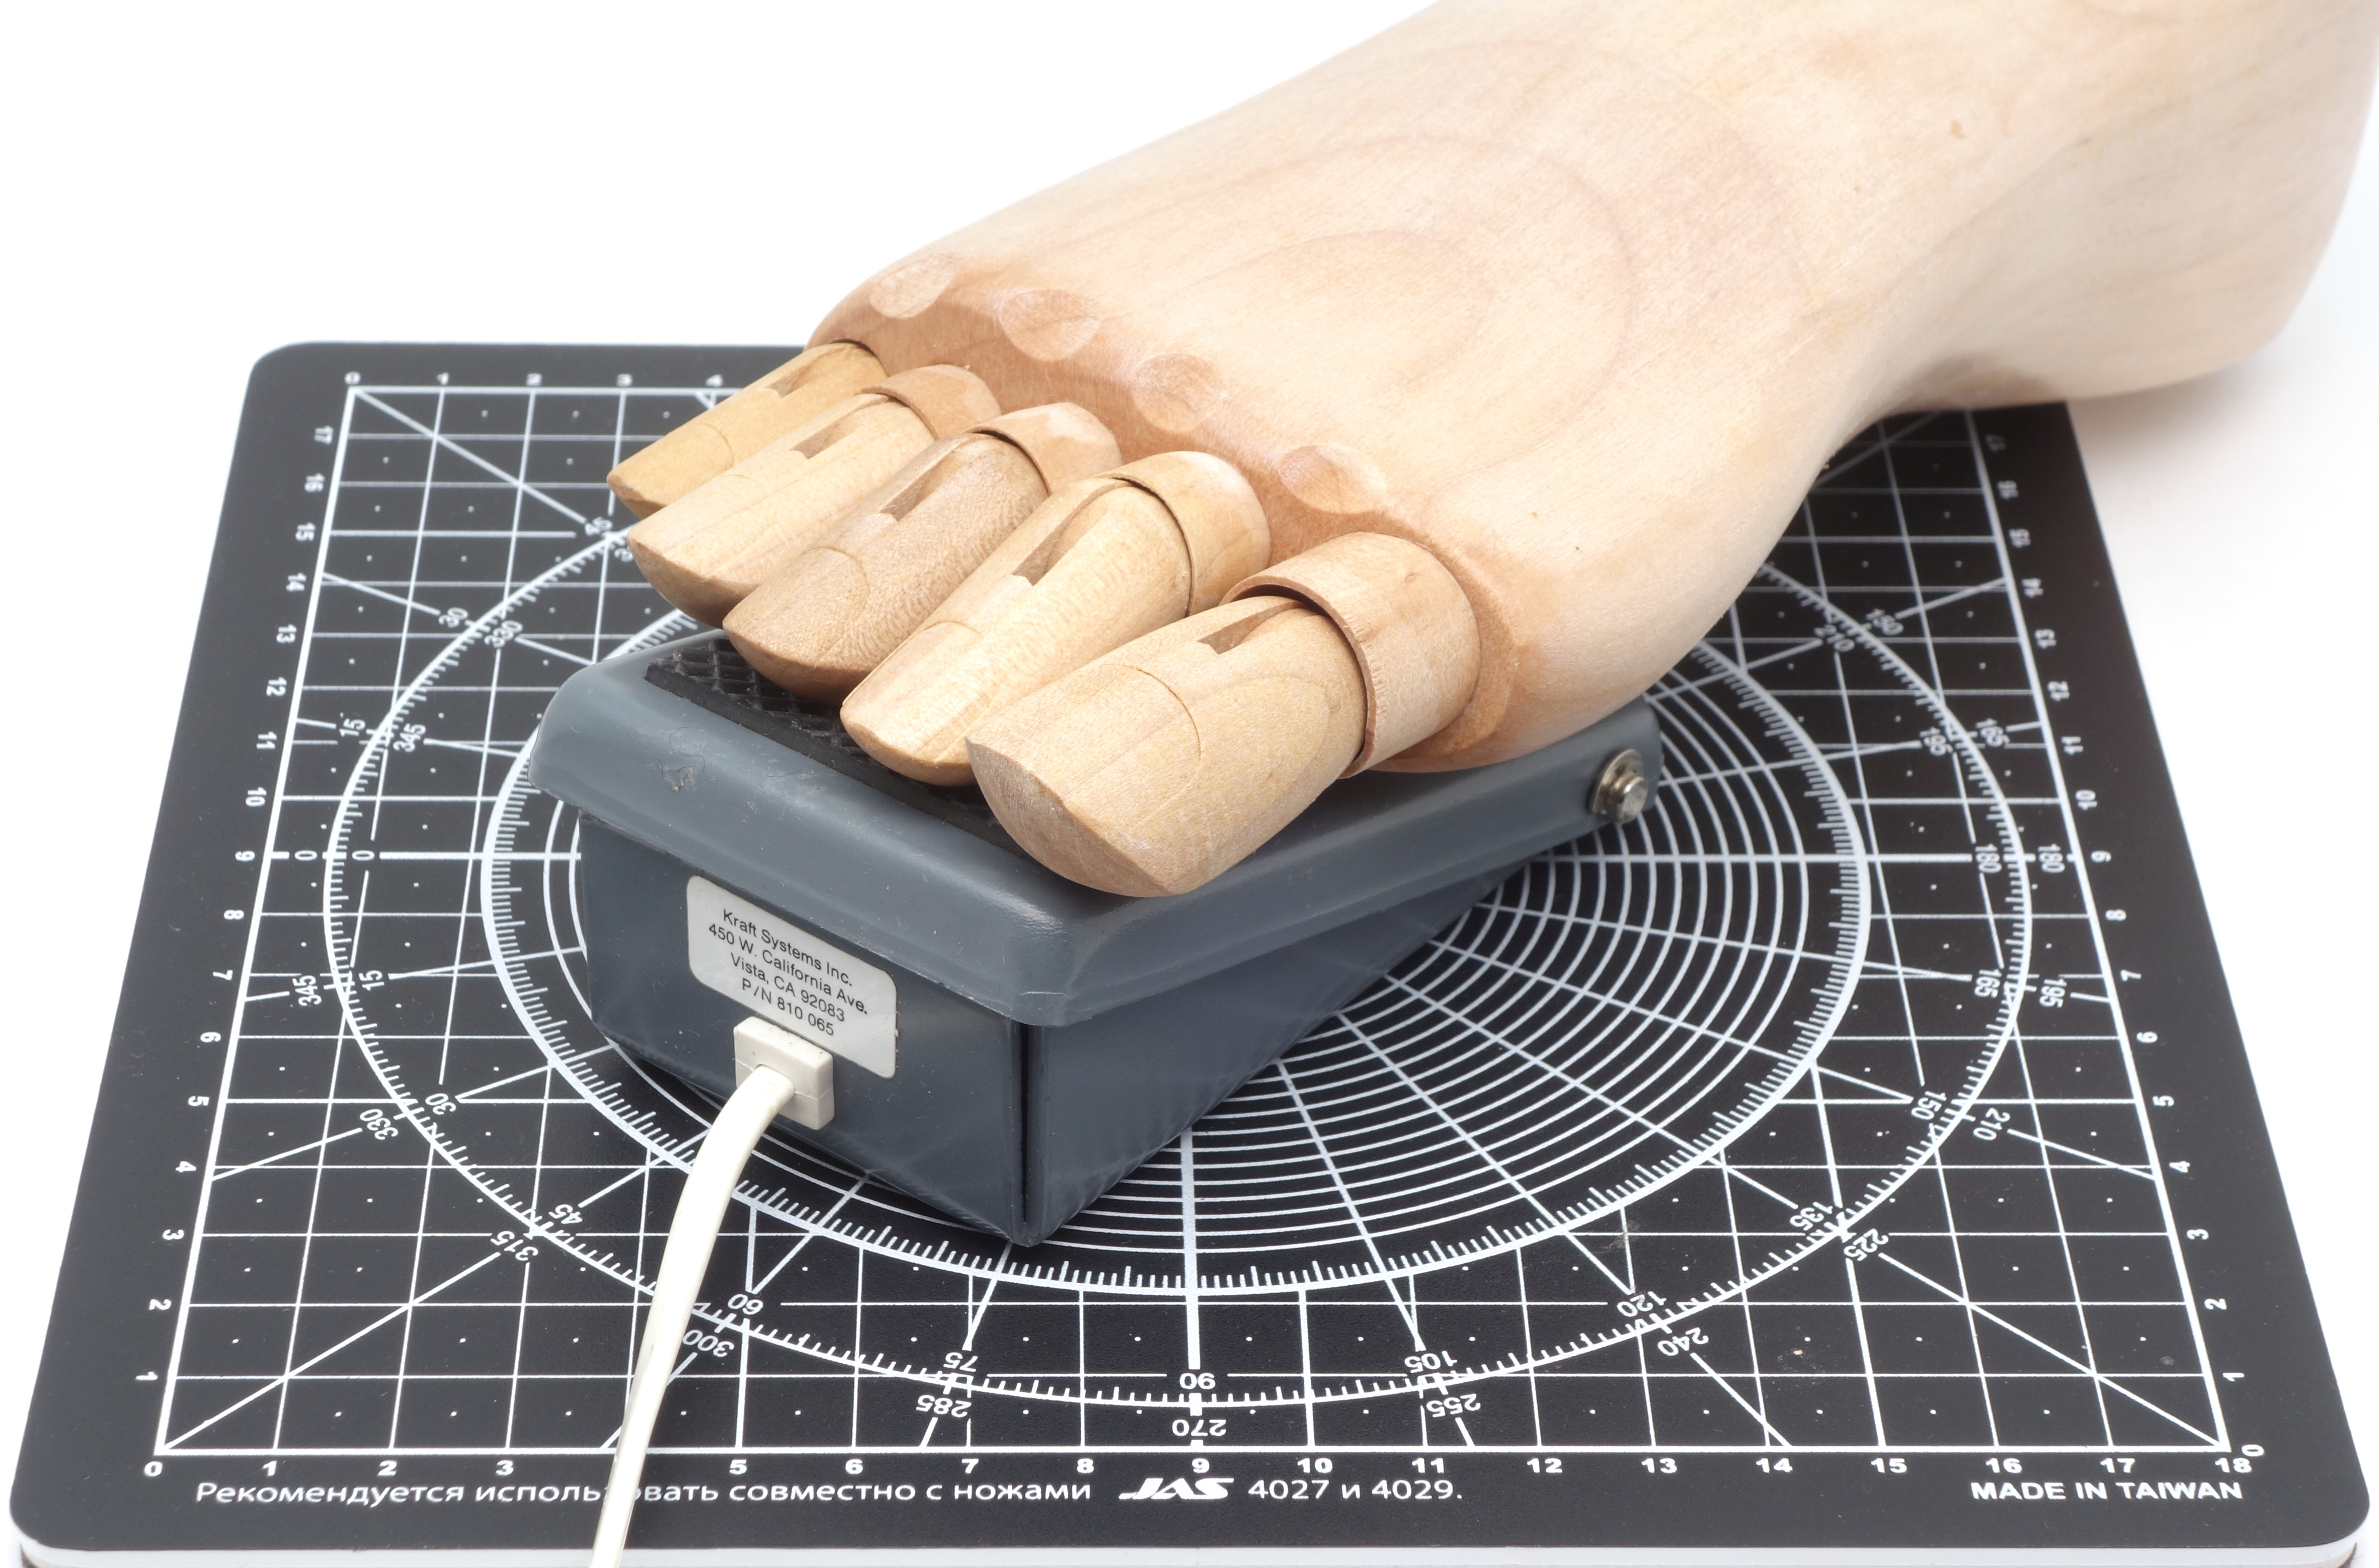
\includegraphics[scale=0.22]{1990_kraft_toptrack/pedal_foot_30.jpg}
    \caption{Kraft trackball pedal}
    \label{fig:KraftPedal}
\end{figure}

\begin{figure}[h]
    \centering
    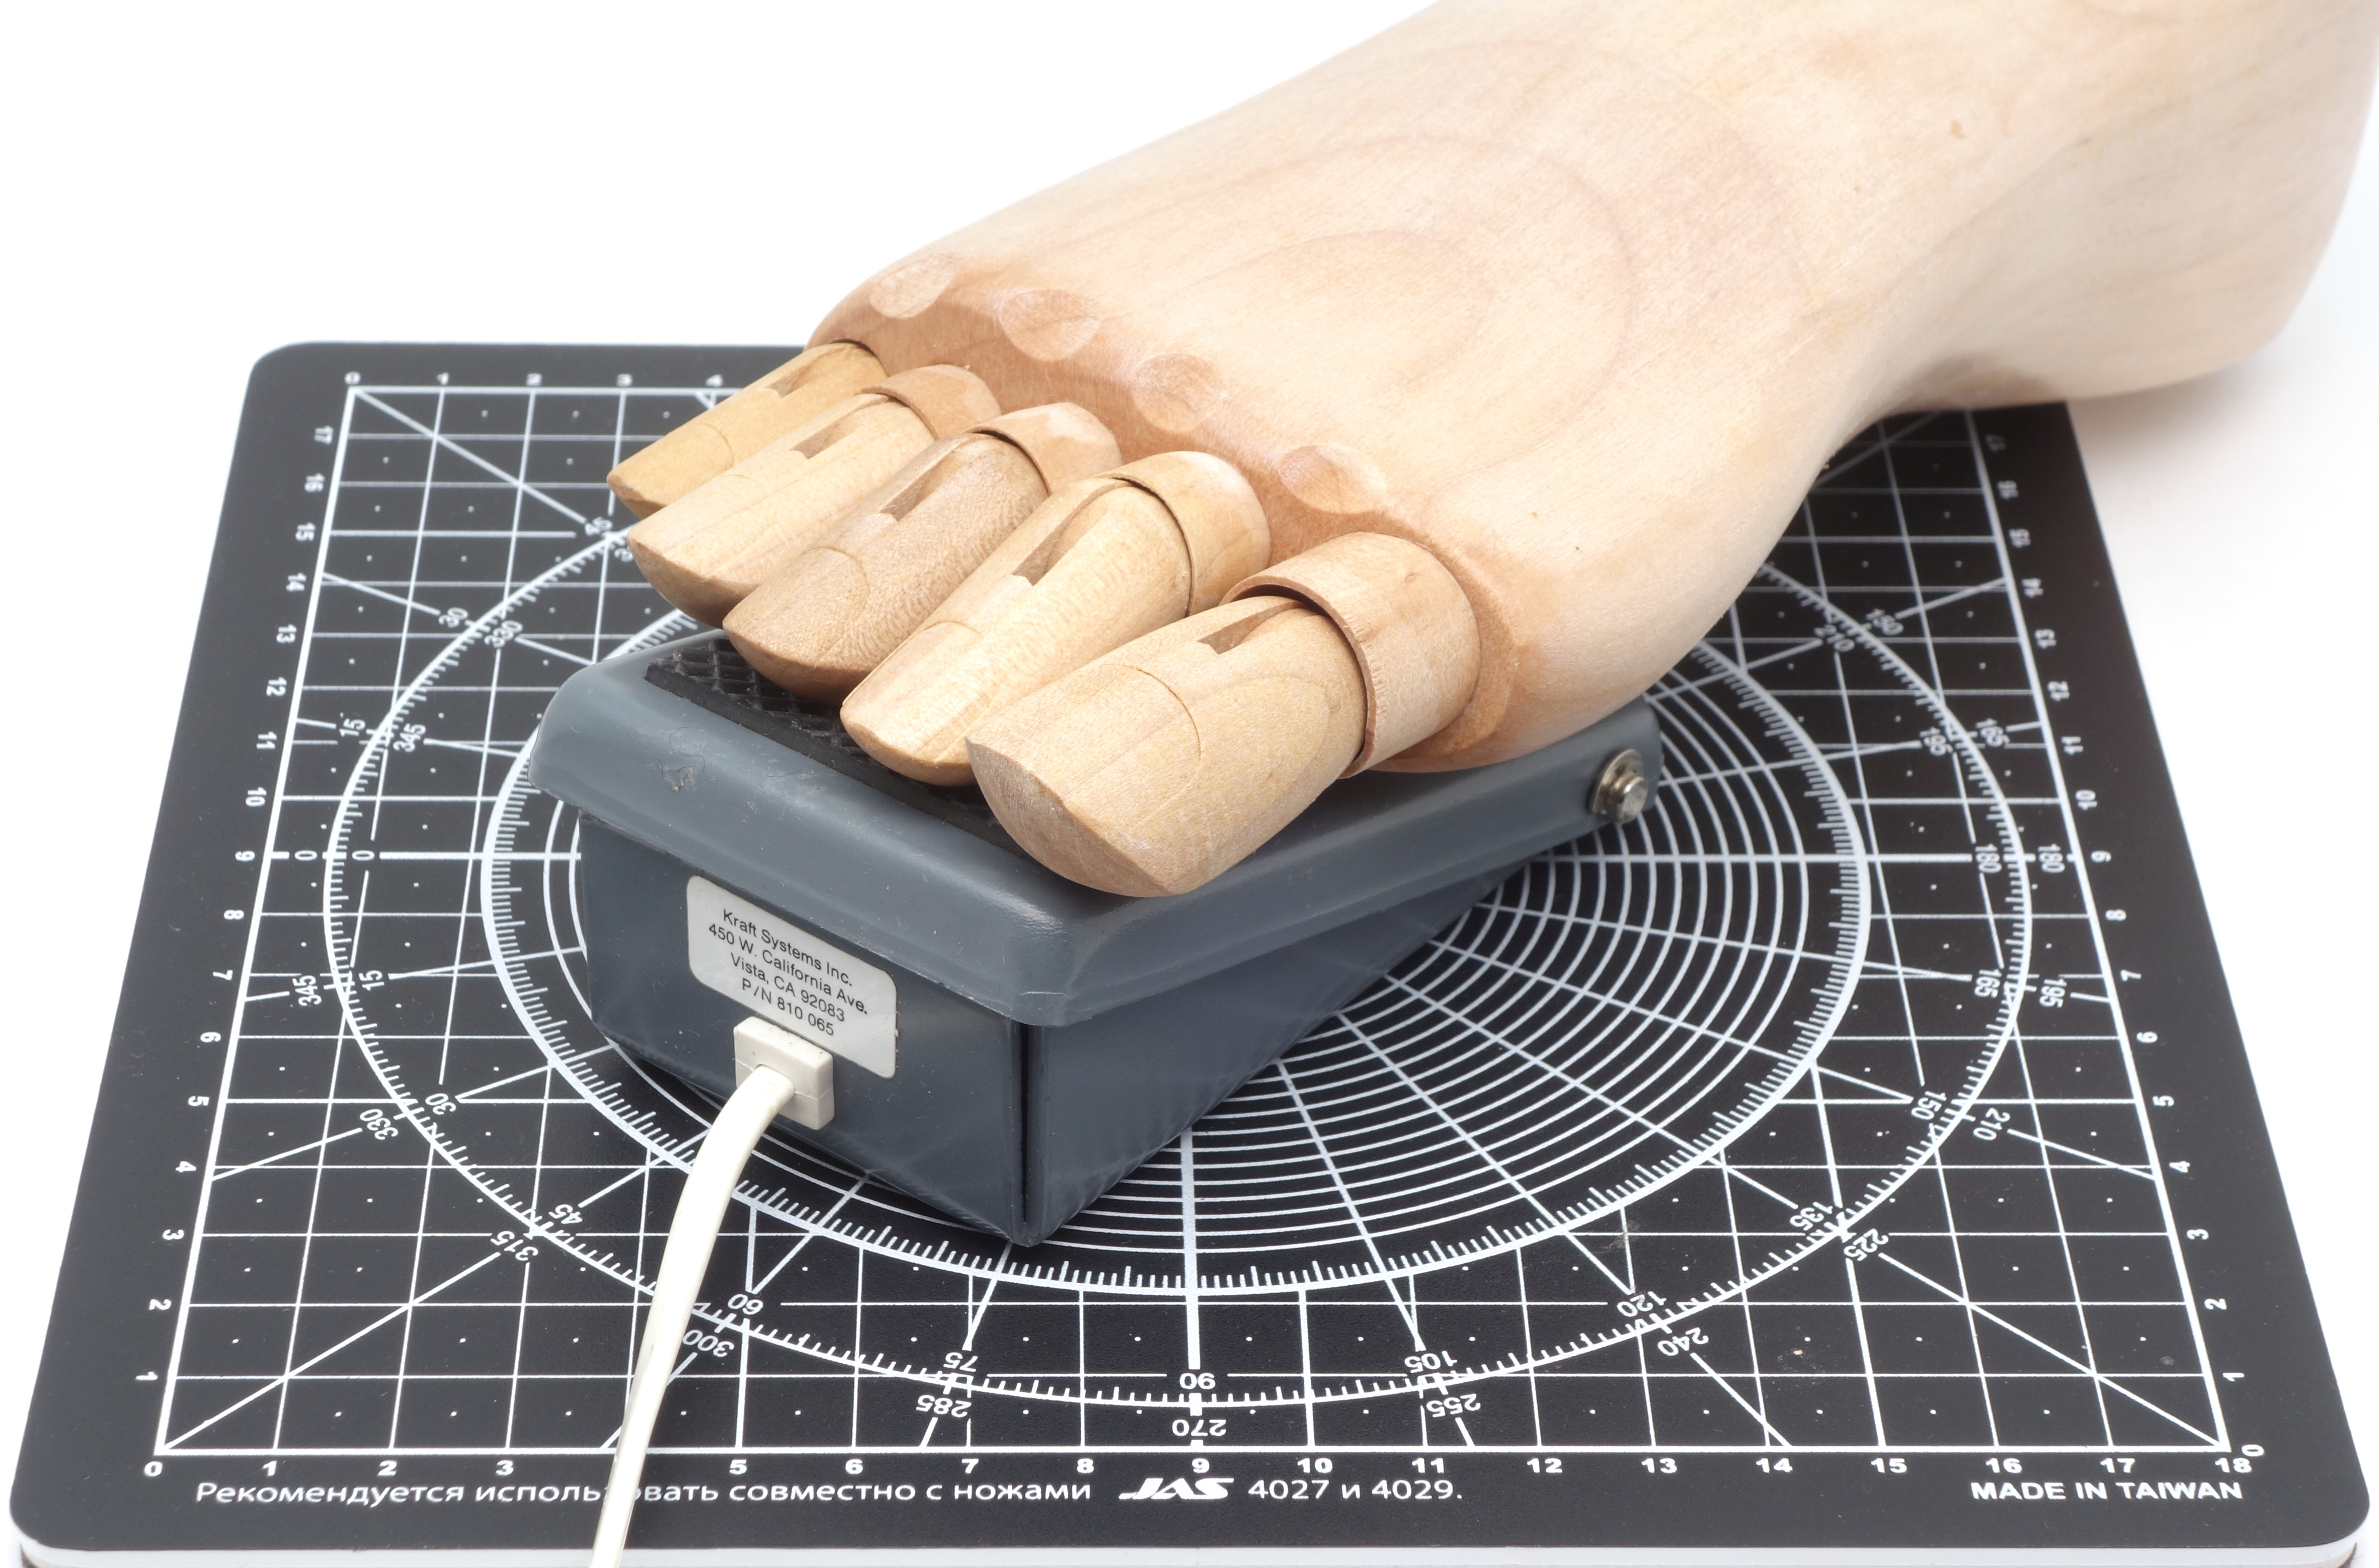
\includegraphics[scale=0.25]{1990_kraft_toptrack/pedal_foot_30.jpg}
    \caption{Kraft TopTrak pedal with a human foot model}
    \label{fig:TopTrakPedalFoot}
\end{figure}

Trackball internals are shown on figure \ref{fig:KraftInside}. As you can see, technically, this is a standard positioning device made according to the optmichanic scheme. The FCC code confirms that Trackball was developed by the American company Kraft Systems in 1989.

\begin{figure}[h]
    \centering
    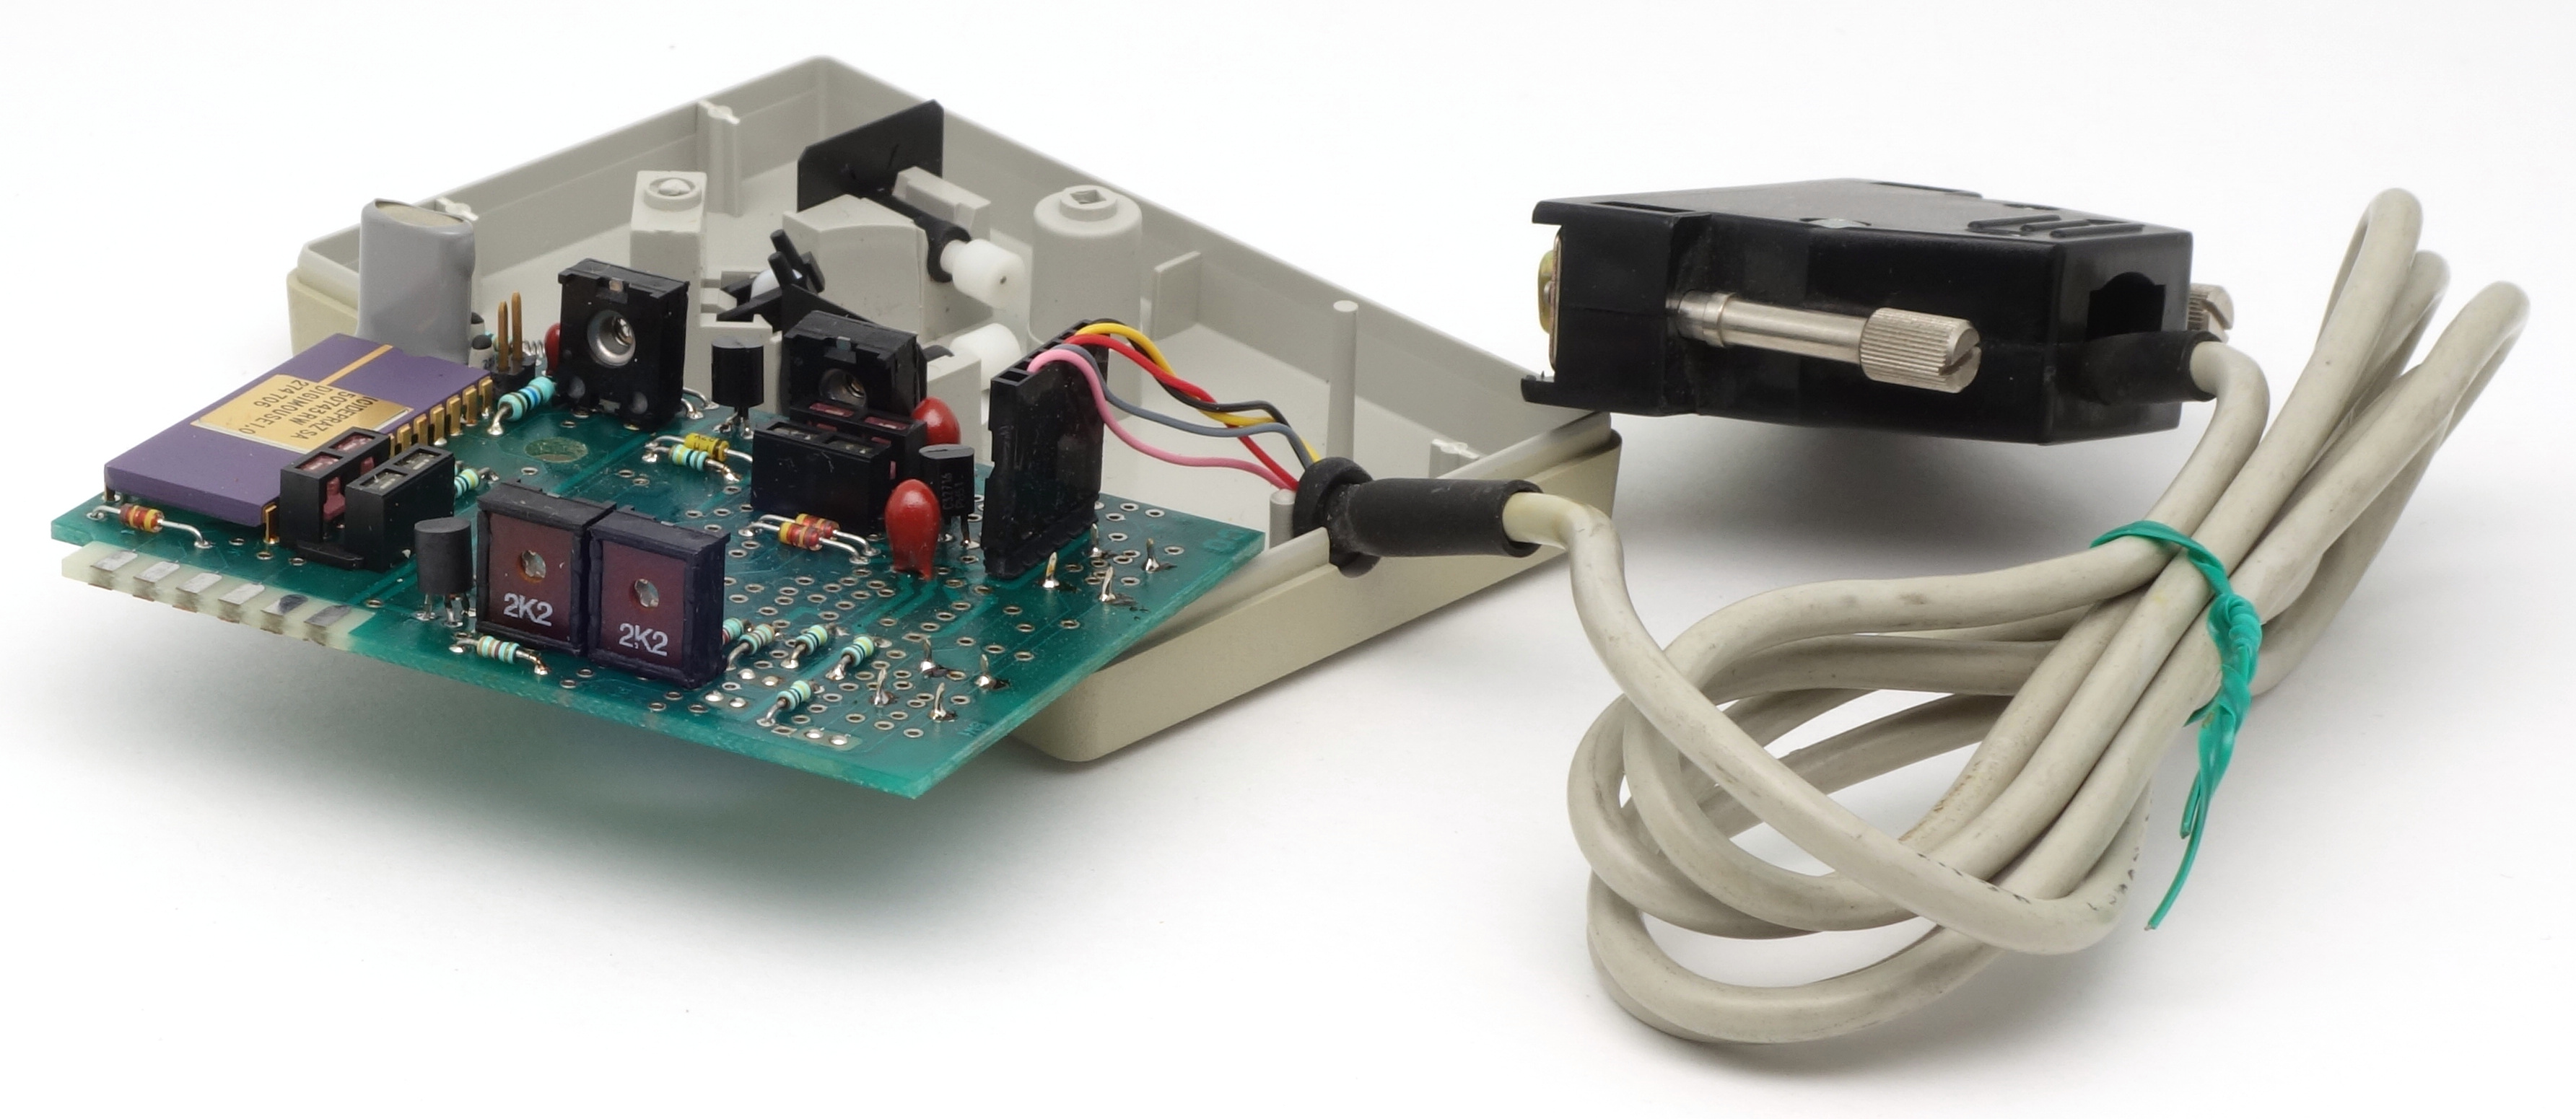
\includegraphics[scale=0.6]{1989_kraft_trackball/inside_30.jpg}
    \caption{Kraft trackball disassembled}
    \label{fig:KraftInside}
\end{figure}

The software supplied with this trackball allows you to use it both with the applications controlled by the mouse and with applications designed for keyboard control. The driver allows you to configure speed, detection of serial ports and some other elements. In addition, Kraft Trackball can be used with a 9-pin connector and a 25-pin connector \cite{Hudnall}.

\begin{thebibliography}{9}
\bibitem{triple} Lennard V. Trackball Round-Up. ATARI/P\&G/CONTRIVER/MCS/MARCONI/KRAFT Trackballs // Music technology, December 1990. -- P. 42--47. \url{http://www.muzines.co.uk/articles/trackball-round-up/462}

\bibitem{Hudnall} Hudnall M. Kraft Trackball // Compute, August 1991. - P. 42. \url{https://www.atarimagazines.com/compute/issue132/42_Kraft_Trackball.php}

\bibitem{kraftwithpedal} Unger T. Kraft Trackball // PC Magazine, V. 9, No. 14, August 1990. - P. 249-251. \url{https://books.google.by/books?id=cSMUxSP5pKgC&lpg=PP1&pg=PT253#v=onepage&q&f=false}
\end{thebibliography}
\end{document} 
